\documentclass{article}

\PassOptionsToPackage{numbers,sort&compress}{natbib}
\usepackage[final]{neurips}

\usepackage[utf8]{inputenc}
\usepackage[T1]{fontenc}
\usepackage{amsmath,amsfonts}
\usepackage{booktabs}
\usepackage{graphicx}
\usepackage{hyperref}
\usepackage{microtype}
\usepackage{nicefrac}
\usepackage{tikz}
\usepackage{url}
\usepackage{xcolor}
\usetikzlibrary{arrows.meta}

\newcommand{\drafttodo}[1]{\textcolor{red!70!black}{\textbf{Draft note:} #1}}

\title{BirdGEN: Conditional Bird-Song Spectrogram Generation for Rare Species Classification}

\author{%
  Shenghao Jin \quad Harvey Li \quad Vincent Wang\\
  Department of Electrical and Computer Engineering, University of Toronto\\
  {\small\texttt{shenghao.jin@mail.utoronto.ca} \quad
  \texttt{harv.li@mail.utoronto.ca}\\
  \texttt{vz.wang@mail.utoronto.ca}}
}

\begin{document}

\maketitle

\begin{abstract}
BirdGEN investigates whether class-conditional spectrogram generation can
improve bird-species classification when labeled data are limited.  We use
recording-isolated log-mel preprocessing, Residual CNN and CRNN classifiers,
and a progressively refined conditional VAE.  With 50 real training examples
per species, adding 200 VAE-v3 samples per species increased mean held-out
macro-F1 from 84.75\% to 87.69\%.  VAE-v3 also achieved a test reconstruction
MSE of 0.0281.  These results support downstream utility in the studied
label-scarcity setting, but do not alone establish perceptual audio realism.
\end{abstract}

\section*{Attestation of Teamwork}
Shenghao Jin contributed to data preparation and the conditional VAE. Harvey
Li contributed to data preparation, the Residual CNN and CRNN classifiers,
the low-resource augmentation experiment, and is responsible for the matched
VAE--Diffusion timing comparison. Vincent Wang developed and evaluated the conditional Diffusion
model. All members contributed to the preparation and revision of the final
report.

\section{Introduction and Problem Formulation}

Field recordings are expensive to collect and annotate, so conditional
generation may provide additional labeled training examples.  Given a species
label $y$ and latent variable $z$, a generator produces a spectrogram
$\hat{x}=G(z,y)$. VAEs provide tractable encoding and one-pass decoding
\cite{kingma2014aevb}, while conditional VAEs incorporate the requested class
\cite{sohn2015cvae}. Although rare-species recognition is the intended
application, our experiment simulates \emph{label scarcity} for three project
species using generators pretrained on the full training split; it is not an
unseen-species experiment.

Our primary question is whether generated samples improve a newly initialized
classifier evaluated on fixed, real, held-out recordings. The endpoint is
$\Delta F1=F1_{\mathrm{real+generated}}-F1_{\mathrm{real-only}}$, using
macro-F1 to weight the three species equally. The secondary question compares
VAE and Diffusion sample quality and equal-count generation time. Quality,
downstream utility, and runtime are kept as separate outcomes.

\section{Data Preparation}

The audited subset contains 3,347 three-second clips from 310 source recording
IDs: 1,017 American Robin, 1,074 Northern Cardinal, and 1,256 Song Sparrow.
Grouping by recording ID prevents clips from the same recording from crossing
train, validation, and test. Historical VAE experiments used 2,339/519/489
clips; the later \texttt{content\_safe\_v2} split removes 24 duplicate training
rows and contains 2,315/519/489 clips. No identified exact duplicate reaches
test, and the low-resource experiment uses the content-safe version.

Audio is mono at 22.05~kHz and converted to $128\times128$ log-mel
spectrograms using a 1,024-point FFT and hop length 512. The VAE uses
training-set global standardization, whereas the maintained classifier maps
each clip's relative 80-dB range to $[-1,1]$; an adapter converts VAE outputs
to the classifier scale.

\section{System Design and Models}

Figure~\ref{fig:pipeline} shows the matched evaluation path. Every downstream
condition trains a fresh CRNN and uses the same real test set.

\begin{figure}[t]
  \centering
  \resizebox{\linewidth}{!}{%
  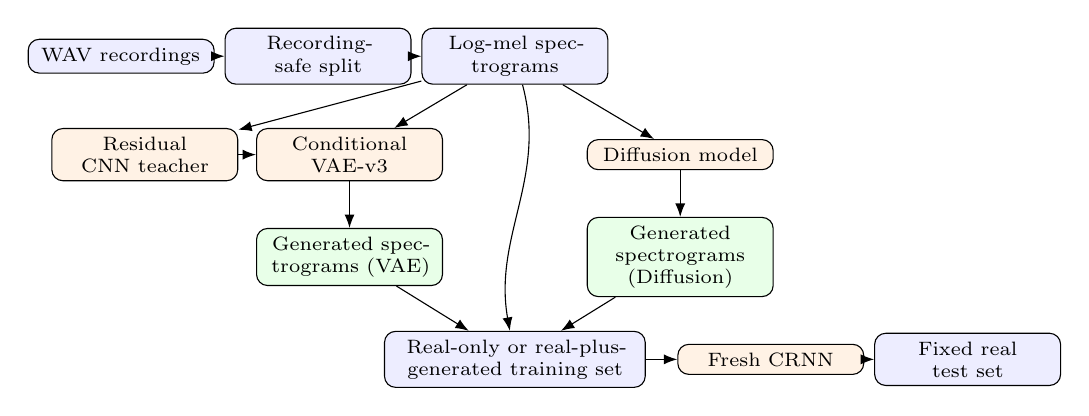
\begin{tikzpicture}[
    block/.style={draw,rounded corners,align=center,inner sep=3pt,
                  text width=2.15cm,font=\scriptsize},
    data/.style={block,fill=blue!7},
    model/.style={block,fill=orange!10},
    generated/.style={block,fill=green!9},
    arrow/.style={-{Latex[length=1.7mm]},thin}
  ]
    \node[data] (wav) at (-5.0,0) {WAV recordings};
    \node[data] (split) at (-2.5,0) {Recording-safe split};
    \node[data] (mel) at (0,0) {Log-mel spectrograms};
    \node[model] (teacher) at (-4.7,-1.25) {Residual CNN teacher};
    \node[model] (vae) at (-2.1,-1.25) {Conditional VAE-v3};
    \node[model] (diff) at (2.1,-1.25) {Diffusion model};
    \node[generated] (gvae) at (-2.1,-2.55) {Generated spectrograms (VAE)};
    \node[generated] (gdiff) at (2.1,-2.55) {Generated spectrograms (Diffusion)};
    \node[data,text width=3.1cm] (train) at (0,-3.85)
      {Real-only or real-plus-generated training set};
    \node[model] (crnn) at (3.25,-3.85) {Fresh CRNN};
    \node[data] (test) at (5.75,-3.85) {Fixed real test set};
    \draw[arrow] (wav) -- (split);
    \draw[arrow] (split) -- (mel);
    \draw[arrow] (mel) -- (teacher);
    \draw[arrow] (mel) -- (vae);
    \draw[arrow] (teacher) -- (vae);
    \draw[arrow] (mel) -- (diff);
    \draw[arrow] (vae) -- (gvae);
    \draw[arrow] (diff) -- (gdiff);
    \draw[arrow] (gvae) -- (train);
    \draw[arrow] (gdiff) -- (train);
    \draw[arrow] (mel) to[out=-75,in=100] (train);
    \draw[arrow] (train) -- (crnn);
    \draw[arrow] (crnn) -- (test);
  \end{tikzpicture}}
  \caption{BirdGEN pipeline. Both generated-spectrogram branches feed the same
  downstream-classifier protocol.}
  \label{fig:pipeline}
\end{figure}

\subsection{Classifiers}

The 1.66-M-parameter Residual CNN uses six residual blocks and global
average/max pooling. Its frozen features and logits guide VAE-v3; its agreement
is therefore a consistency diagnostic, not independent realism evidence. The
selected 404-k-parameter CRNN combines convolutional spectral features with a
bidirectional GRU and temporal pooling \cite{cakir2017crnn}. Frozen CRNN scores
are diagnostics, while freshly initialized CRNNs provide the primary
augmentation evidence.

\subsection{Conditional VAE Evolution}

V1 established a CVAE baseline with a flat 128-value latent, label
concatenation, and MSE+KL loss, but its samples blurred narrow calls. V2 used a
$16\times8\times8$ spatial latent, residual FiLM conditioning
\cite{perez2018film}, resize-convolution, detail-aware losses, and
species-matched posterior statistics to preserve time--frequency location. V3
increased the latent to $16\times16\times16$, added free bits and frozen
classifier feature/label consistency, and sampled from 256 posterior anchors
per species. These changes targeted fine transients, species cues, and the
mismatch between the standard-normal prior and the learned posterior. Because
several components changed together, the versions are an engineering
progression rather than a controlled ablation.

VAE-v3 has 5.37~M parameters. Species embeddings modulate residual blocks with
FiLM, and the objective combines event-weighted and multiscale reconstruction,
time/frequency gradients, free-bits KL, and frozen-classifier consistency:
\begin{equation}
\mathcal{L}=\mathcal{L}_{\mathrm{event}}+0.25\mathcal{L}_{\mathrm{ms}}
+0.60(\mathcal{L}_{\Delta t}+\mathcal{L}_{\Delta f})
+\beta\mathcal{L}_{\mathrm{KL,free}}
+s_{\mathrm{cls}}[0.08\mathcal{L}_{\mathrm{feat}}+0.03\mathcal{L}_{\mathrm{label}}].
\label{eq:vae-loss}
\end{equation}
Multiscale and feature-space terms are motivated by
\cite{mathieu2016multiscale,johnson2016perceptual}; free bits follow
\cite{kingma2016iaf}. For generation, V3 perturbs a class-matched posterior
anchor rather than drawing independently from a standard-normal prior, an idea
related in motivation to mixture priors such as VampPrior
\cite{tomczak2018vampprior}.

\subsection{Diffusion Model}
% Intentionally left blank until the canonical Diffusion implementation is supplied.

\section{Experimental Methodology}

Classifier architectures were selected on validation data across seeds 42,
123, and 777, then evaluated on held-out test recordings. VAE evidence is
separated into paired deterministic reconstruction, unpaired generated-sample
quality, and downstream classifier utility. To address the presentation
feedback, each frozen generated sample was compared with its nearest
same-species test spectrogram in the standardized-logmel domain, with a
leave-one-out real-test reference. The test set was used only for this final
evaluation; low MSE can also indicate copying or limited diversity.

For the primary experiment, each fresh CRNN sees 50 real examples per species.
Three real-subset seeds crossed with three classifier seeds give nine matched
blocks. Ratios of 50, 100, or 200 generated examples per species are selected
using real validation data; only real-only and the selected ratio reach the
fixed real test set. Architecture, augmentation, and optimizer-step budget are
matched. For runtime, both generators will produce 600 spectrograms on the same
GPU, precision, and batch size after warm-up; generator-only and waveform
decoding time will be reported separately.

\section{Experimental Results}

\paragraph{Classifier and VAE diagnostics.}
The selected CRNN obtained 90.16\% macro-F1 on 489 held-out clips. Across VAE
versions, deterministic test reconstruction MSE decreased from 0.1533 (V1) to
0.0654 (V2) and 0.0281 (V3); V3 test MAE was 0.1261 and spectral convergence
was 0.1794. These paired reconstruction values do not measure the distance
between independently generated and real examples. V3 generated-sample
time-detail ratios were 0.770--0.833 and frequency-detail ratios were
0.518--0.575, showing stronger remaining smoothing along frequency.

\begin{figure}[t]
  \centering
  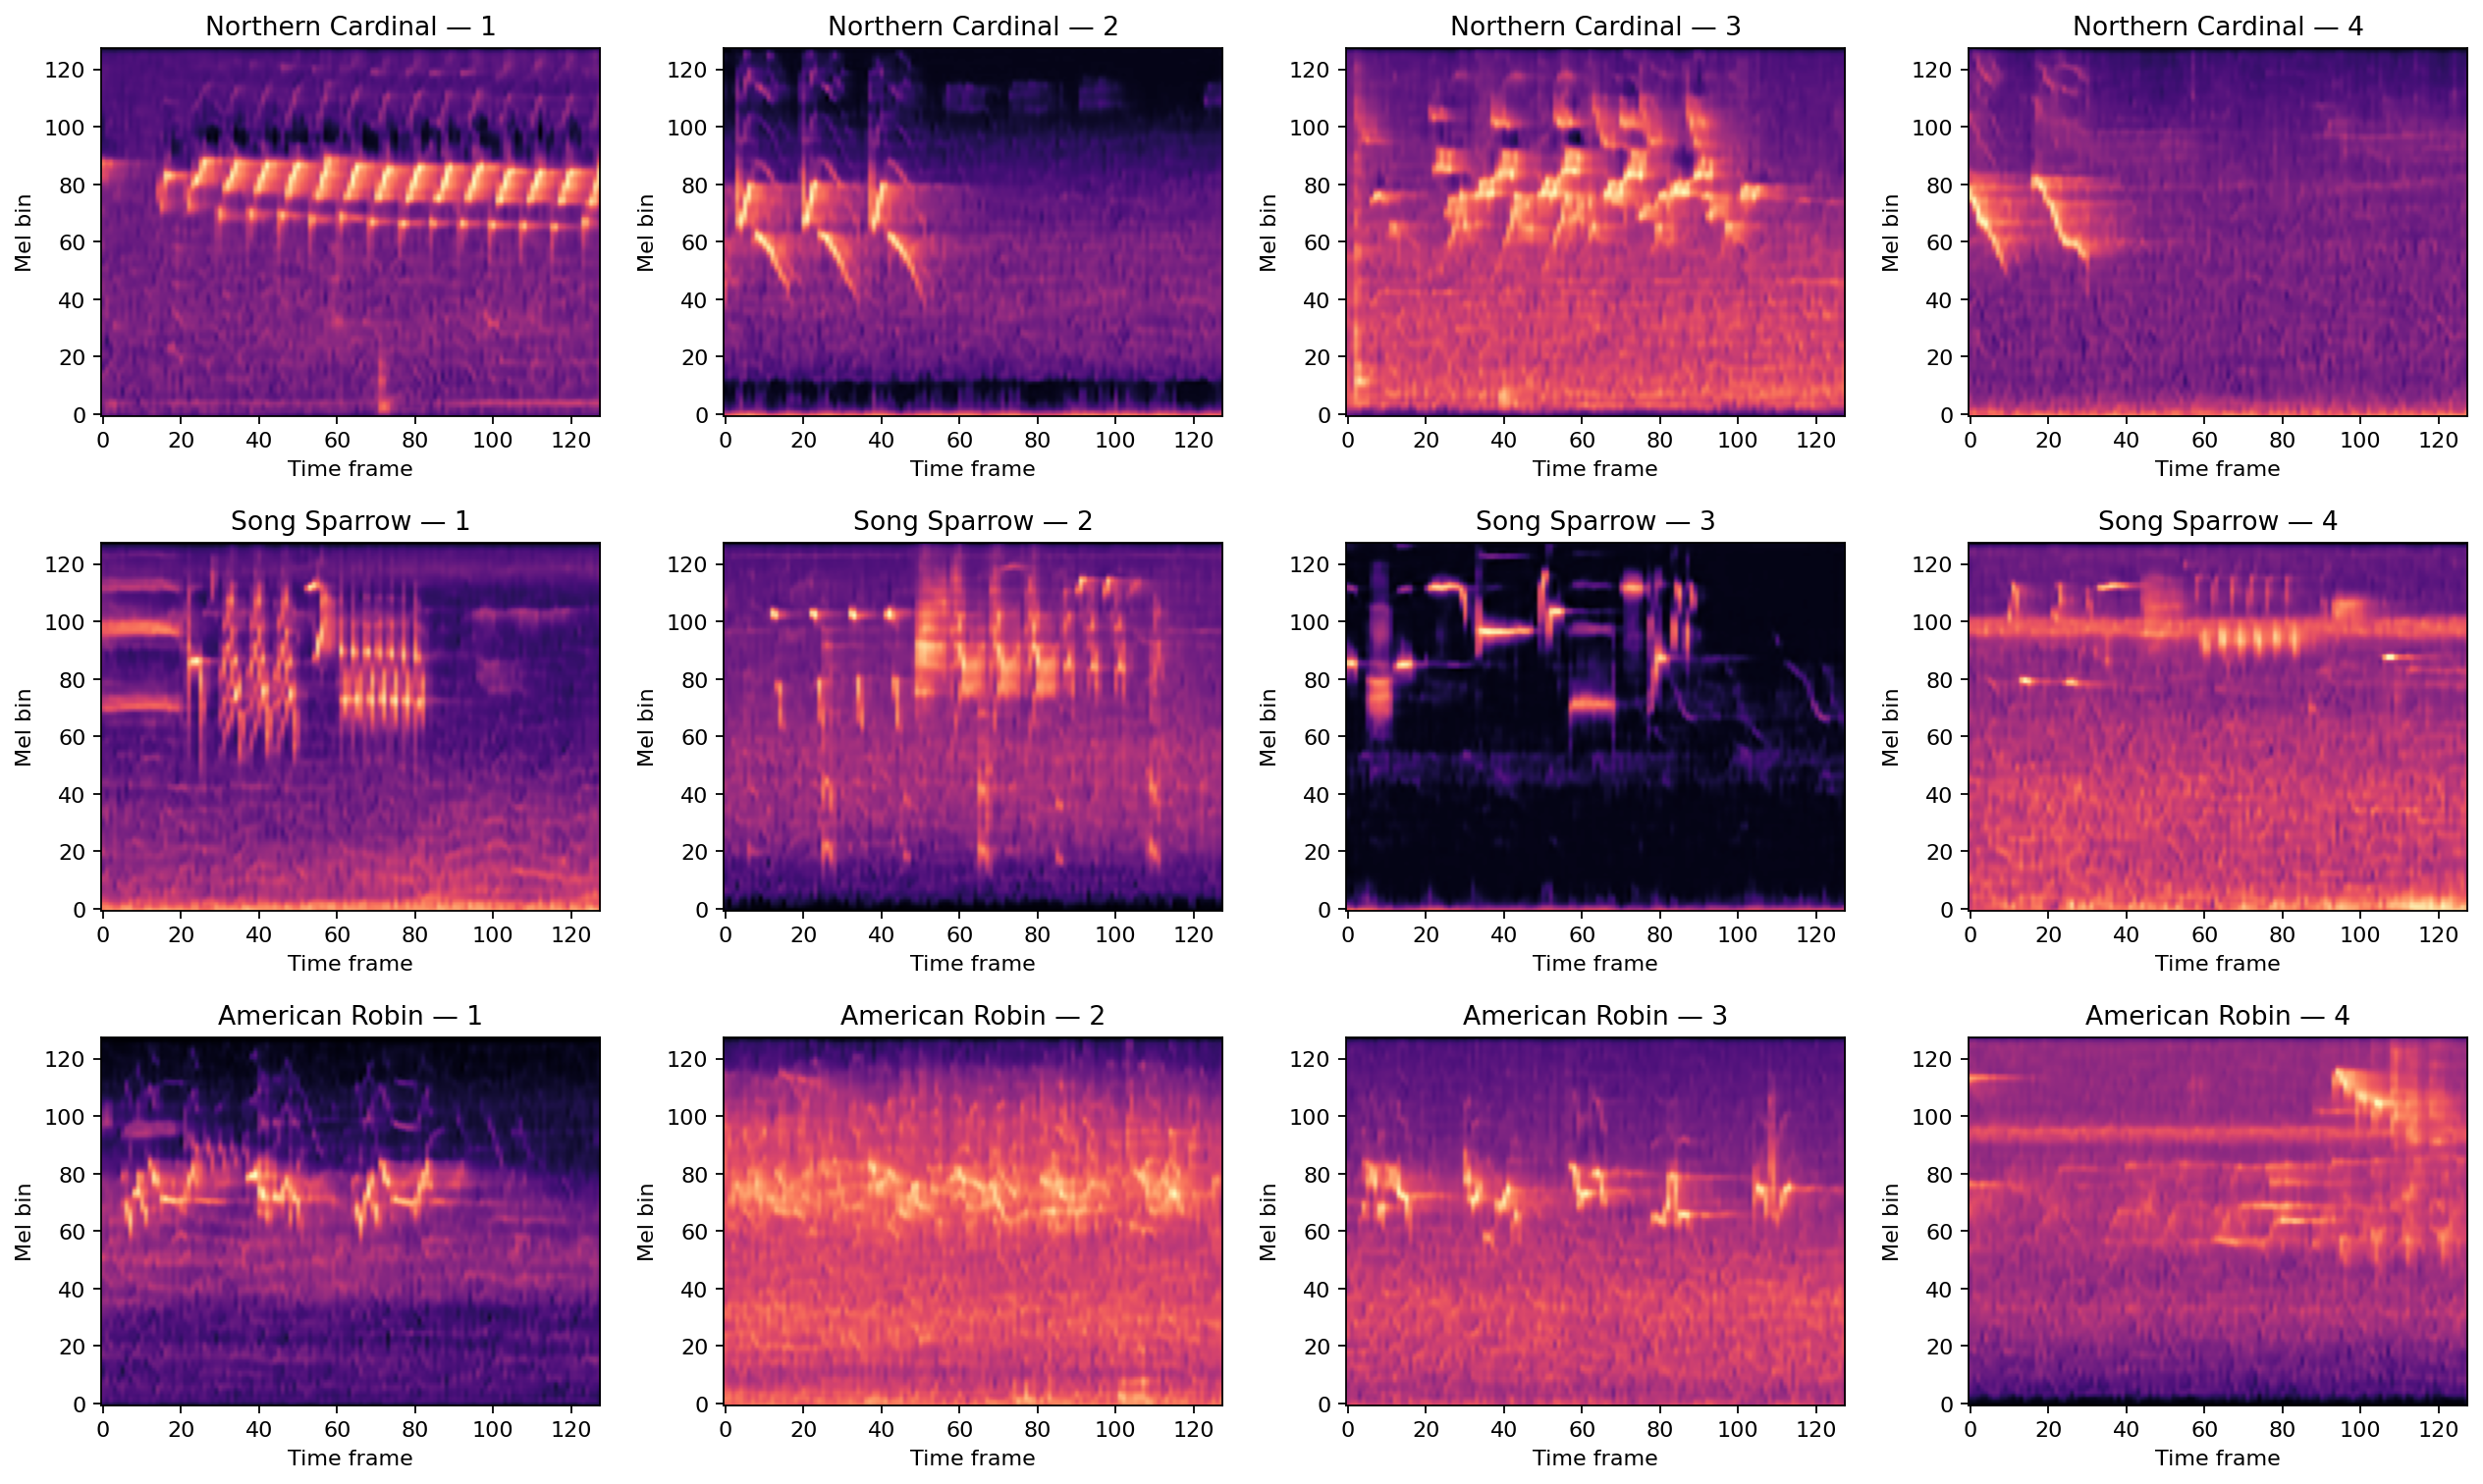
\includegraphics[width=0.93\linewidth]{../../reports/vae/conditional_vae_v3/conditional_samples.png}
  \caption{VAE-v3 posterior-anchor samples for Northern Cardinal (top), Song
  Sparrow (middle), and American Robin (bottom). The final version will use a
  shared-scale $3\times3$ grid.}
  \label{fig:vae-samples}
\end{figure}

The 48 historical samples achieved 100\% target agreement under the Residual
teacher (mean confidence 0.915), but that classifier also contributes to
Eq.~\eqref{eq:vae-loss}; the result is not an independent realism score.
For the separately verified seed-42 notebook pool (16 samples/species), the
same-species generated-to-test nearest-neighbor MSE was 0.5120 on average
(SD 0.1998; median 0.4501; IQR 0.3878--0.6231), versus 0.3350 for the
leave-one-out real-to-real reference (SD 0.1419; median 0.3185; IQR
0.2368--0.4154). Generated/real means were 0.4308/0.3237 for American Robin,
0.5579/0.3650 for Northern Cardinal, and 0.5474/0.3175 for Song Sparrow.
These are unpaired pixel-space summaries (48 versus 489 queries), not a
perceptual-realism or waveform-quality score; nearest-neighbor MSE can reward
copying. This hash-recorded diagnostic used the original notebook sampler at
temperature 0.35 with a train-only posterior bank, not Harvey's corrected
canonical pool.

\paragraph{Low-resource augmentation.}
\begin{table}[t]
  \caption{Matched CRNN performance on the fixed real test set (nine blocks).}
  \label{tab:low-resource}
  \centering
  \small
  \begin{tabular}{@{}lrrr@{}}
    \toprule
    Training condition & Mean macro-F1 & Paired change & Positive blocks \\
    \midrule
    50 real/species & 84.75\% & reference & -- \\
    $+$200 VAE-v3/species & \textbf{87.69\%} & \textbf{$+2.93$ pp} & \textbf{8/9} \\
    \bottomrule
  \end{tabular}
\end{table}

Adding 200 VAE-v3 samples per species increased mean test macro-F1 by 2.93
percentage points; the descriptive paired bootstrap interval was
$[1.43,4.54]$ points. This is the strongest current evidence that generated
samples add useful training variation. It is a transfer-augmentation result:
the generator was pretrained with more real data than each downstream CRNN.
\drafttodo{Insert the matched VAE--Diffusion quality and 600-sample timing
comparison, including the absolute gap and Diffusion/VAE ratio.}

\section{Discussion}

VAE-v3 augmentation improved a fresh classifier under matched label scarcity,
but the conclusion is narrower than the title's intended rare-species setting.
Reconstruction MSE rewards pixel proximity, the Residual teacher is coupled to
V3 training, and a closed-set classifier cannot reject unknown or noisy audio.
Moreover, log-mel generation omits phase; Griffin--Lim is a separate waveform
bottleneck, so listening or vocoder evaluation is still required
\cite{bhatia2022birdsong}. The secondary VAE--Diffusion conclusion must wait
for the same generated-to-test, diversity, and timing protocol for both models.

\section{Conclusion}

BirdGEN demonstrates that conditional spectrogram generation can be useful
beyond visual plausibility: VAE-v3 augmentation improved held-out macro-F1 by
2.93 points in the recorded experiment. Successive VAE revisions reduced test
reconstruction MSE to 0.0281 while better preserving local detail. The result
supports full-data-pretrained transfer augmentation under simulated label
scarcity; verified generated-to-test MSE and an equal-count VAE--Diffusion
quality/runtime comparison remain required for the final report.

\clearpage
\begin{thebibliography}{99}
\small

\bibitem{kingma2014aevb}
D. P. Kingma and M. Welling, ``Auto-Encoding Variational Bayes,'' in
\emph{Proc. Int. Conf. Learn. Represent. (ICLR)}, 2014.

\bibitem{sohn2015cvae}
K. Sohn, H. Lee, and X. Yan, ``Learning structured output representation using
deep conditional generative models,'' in \emph{Adv. Neural Inf. Process.
Syst.}, vol. 28, pp. 3483--3491, 2015.

\bibitem{cakir2017crnn}
E. Cakir, G. Parascandolo, T. Heittola, H. Huttunen, and T. Virtanen,
``Convolutional recurrent neural networks for polyphonic sound event
detection,'' \emph{IEEE/ACM Trans. Audio, Speech, Lang. Process.}, vol. 25,
no. 6, pp. 1291--1303, 2017.

\bibitem{perez2018film}
E. Perez, F. Strub, H. de Vries, V. Dumoulin, and A. Courville, ``FiLM: Visual
reasoning with a general conditioning layer,'' in \emph{Proc. AAAI Conf.
Artif. Intell.}, vol. 32, no. 1, pp. 3942--3951, 2018.

\bibitem{mathieu2016multiscale}
M. Mathieu, C. Couprie, and Y. LeCun, ``Deep multi-scale video prediction
beyond mean square error,'' in \emph{Proc. ICLR}, 2016.

\bibitem{kingma2016iaf}
D. P. Kingma, T. Salimans, R. Jozefowicz, X. Chen, I. Sutskever, and M.
Welling, ``Improved variational inference with inverse autoregressive flow,''
in \emph{Adv. Neural Inf. Process. Syst.}, vol. 29, pp. 4743--4751, 2016.

\bibitem{johnson2016perceptual}
J. Johnson, A. Alahi, and L. Fei-Fei, ``Perceptual losses for real-time style
transfer and super-resolution,'' in \emph{Computer Vision--ECCV}, pp.
694--711, 2016.

\bibitem{tomczak2018vampprior}
J. Tomczak and M. Welling, ``VAE with a VampPrior,'' in \emph{Proc. AISTATS},
PMLR, vol. 84, pp. 1214--1223, 2018.

\bibitem{bhatia2022birdsong}
R. R. Bhatia and T. H. Kinnunen, ``An initial study on birdsong re-synthesis
using neural vocoders,'' in \emph{Speech and Computer}, pp. 64--74, 2022.

\end{thebibliography}

\clearpage
\appendix
\section{Supplementary Reproducibility Notes}

VAE-v3 used AdamW with learning rate $2\times10^{-4}$, batch size 24, a
20-epoch KL warm-up, and checkpoint selection by the complete validation
objective. The portable pool generator now applies the notebook's sampling
temperature 0.35 explicitly; however, previously generated untracked pools do
not contain a generation-code hash, so their exact formula remains unverified.
The reported generated-to-test MSE instead uses a separate, hash-recorded
seed-42 pool reconstructed with the original notebook, 16 samples per species,
and the train-only posterior bank. It does not verify the historical three-seed
augmentation pools; the low-resource experiment must still be rerun if the
report claims that it used Harvey's corrected canonical sampler.

For the equal-count timing study, each model will generate 600 spectrograms
(200 per species) in FP32 with batch size 8 on the same hardware. Five warm-up
batches precede at least five synchronized repeats with alternating model
order. Generator-only time is reported separately from common 32-iteration
Griffin--Lim decoding and WAV I/O.

\end{document}
